%%%%%%%%%%%%%%%%%%%%%%%%%%%%%%%%%%%%%%%%%
% Short Sectioned Assignment
% LaTeX Template
% Version 1.0 (5/5/12)

%
% This template has been downloaded from:
% http://www.LaTeXTemplates.com
%
% Original author:
% Frits Wenneker (http://www.howtotex.com)
%
% License:
% CC BY-NC-SA 3.0 (http://creativecommons.org/licenses/by-nc-sa/3.0/)
%
%%%%%%%%%%%%%%%%%%%%%%%%%%%%%%%%%%%%%%%%%

%----------------------------------------------------------------------------------------
%	PACKAGES AND OTHER DOCUMENT CONFIGURATIONS
%----------------------------------------------------------------------------------------

\documentclass[paper=a4, fontsize=11pt]{scrartcl} % A4 paper and 11pt font size

\usepackage{graphicx} 
\usepackage{listings}
\usepackage[T1]{fontenc} % Use 8-bit encoding that has 256 glyphs
\usepackage{fourier} % Use the Adobe Utopia font for the document - comment this line to return to the LaTeX default
\usepackage[english]{babel} % English language/hyphenation
\usepackage{amsmath,amsfonts,amsthm} % Math packages
\usepackage{caption}
\captionsetup{font = {scriptsize}}
\usepackage{lipsum} % Used for inserting dummy 'Lorem ipsum' text into the template
\usepackage{subfigure}
\usepackage{latexsym}
\usepackage{sectsty} % Allows customizing section commands
\allsectionsfont{\centering \normalfont\scshape} % Make all sections centered, the default font and small caps
\usepackage{color} %red, green, blue, yellow, cyan, magenta, black, white
\definecolor{mygreen}{RGB}{28,172,0} % color values Red, Green, Blue
\definecolor{mylilas}{RGB}{170,55,241}
\usepackage{float}
\usepackage{fancyhdr} % Custom headers and footers
\pagestyle{fancyplain} % Makes all pages in the document conform to the custom headers and footers
\fancyhead{} % No page header - if you want one, create it in the same way as the footers below
\fancyfoot[L]{} % Empty left footer
\fancyfoot[C]{} % Empty center footer
\fancyfoot[R]{\thepage} % Page numbering for right footer
\renewcommand{\headrulewidth}{0pt} % Remo\label{\label{key}}ve header underlines
\renewcommand{\footrulewidth}{0pt} % Remove footer underlines
\setlength{\headheight}{13.6pt} % Customize the height of the header
\definecolor{mygreen}{rgb}{0,0.6,0}
\definecolor{mygray}{rgb}{0.5,0.5,0.5}
\definecolor{mymauve}{rgb}{0.58,0,0.82}
\numberwithin{equation}{section} % Number equations within sections (i.e. 1.1, 1.2, 2.1, 2.2 instead of 1, 2, 3, 4)
\numberwithin{figure}{section} % Number figures within sections (i.e. 1.1, 1.2, 2.1, 2.2 instead of 1, 2, 3, 4)
\numberwithin{table}{section} % Number tables within sections (i.e. 1.1, 1.2, 2.1, 2.2 instead of 1, 2, 3, 4)
\newcommand{\mygamma}{\ensuremath{\gamma{}}}
\setlength\parindent{0pt} % Removes all indentation from paragraphs - comment this line for an assignment with lots of text

%----------------------------------------------------------------------------------------
%	TITLE SECTION
%----------------------------------------------------------------------------------------

\newcommand{\horrule}[1]{\rule{\linewidth}{#1}} % Create horizontal rule command with 1 argument of height

\title{	
\normalfont \normalsize 
\textsc{Purdue University} \\ [25pt] % Your university, school and/or department name(s)
\horrule{0.5pt} \\[0.4cm] % Thin top horizontal rule
\huge ECE 637 Laboratory Exercise 9\\ 
\huge Achromatic Baseline JPEG encoding Lab\\% The assignment title
\horrule{2pt} \\[0.5cm] % Thick bottom horizontal rule
}

\author{Tong Shen} % Your name

\date{\normalsize\today} % Today's date or a custom date

\begin{document}

\maketitle % Print the title

%----------------------------------------------------------------------------------------
%	PROBLEM 1
%----------------------------------------------------------------------------------------
\section{Introduction}
Nothing to report for this section. 

\section{ DCT Block Transforms and Quantization}
The source image is first broken into 8x8 blocks. The pixel values Syx in each of these blocks
are then transformed by the FDCT into an 8 x 8 block of 64 DCT coefficients.

\subsection{Code List of Transforming, Quantization and Storing}

\lstset{language=Matlab,%
	%basicstyle=\color{red},
	breaklines=true,%
	morekeywords={matlab2tikz},
	keywordstyle=\color{blue},%
	morekeywords=[2]{1}, keywordstyle=[2]{\color{black}},
	identifierstyle=\color{black},%
	stringstyle=\color{mylilas},
	commentstyle=\color{mygreen},%
	showstringspaces=false,%without this there will be a symbol in the places where there is a space
	numbers=left,%
	numberstyle={\tiny \color{black}},% size of the numbers
	numbersep=9pt, % this defines how far the numbers are from the text
	emph=[1]{for,end,break},emphstyle=[1]\color{red}, %some words to emphasise
	%emph=[2]{word1,word2}, emphstyle=[2]{style},    
}
\begin{lstlisting}[frame=single]

I = imread('img03y.tif');
I = double(I);
I = I - 128;

gamma = 1;
fn = @(x) round(dct2(x.data,[8,8])./(Quant*gamma));
dct_blk = blockproc(I,[8,8],fn);
dct_blk = dct_blk';
[r,c] = size(dct_blk);
fileID = fopen('img03y.dq','w');
fwrite(fileID,r,'integer*2');
fwrite(fileID,c,'integer*2');
fwrite(fileID,dct_blk,'integer*2');
fclose(fileID);

image_1 = readfile('img03y.dq',gamma);

imshow(image_1')
image_different = image_1' - I1;
figure(2)
imshow(image_different)

\end{lstlisting}
\begin{lstlisting}[frame=single]

function [image] = readfile(file,gamma)
run('Qtables');
f = fopen(file,'r');
data = fread(f,'integer*2');
image = reshape(data(3:end),[data(1),data(2)]);
fn = @(x) round(idct2(x.data.*Quant*gamma,[8,8]));
image = blockproc(image,[8,8],fn);
image = image + 128;
image = uint8(image);
end

\end{lstlisting}

\subsection{Result report}
\begin{figure}[H]
	
	\centering
	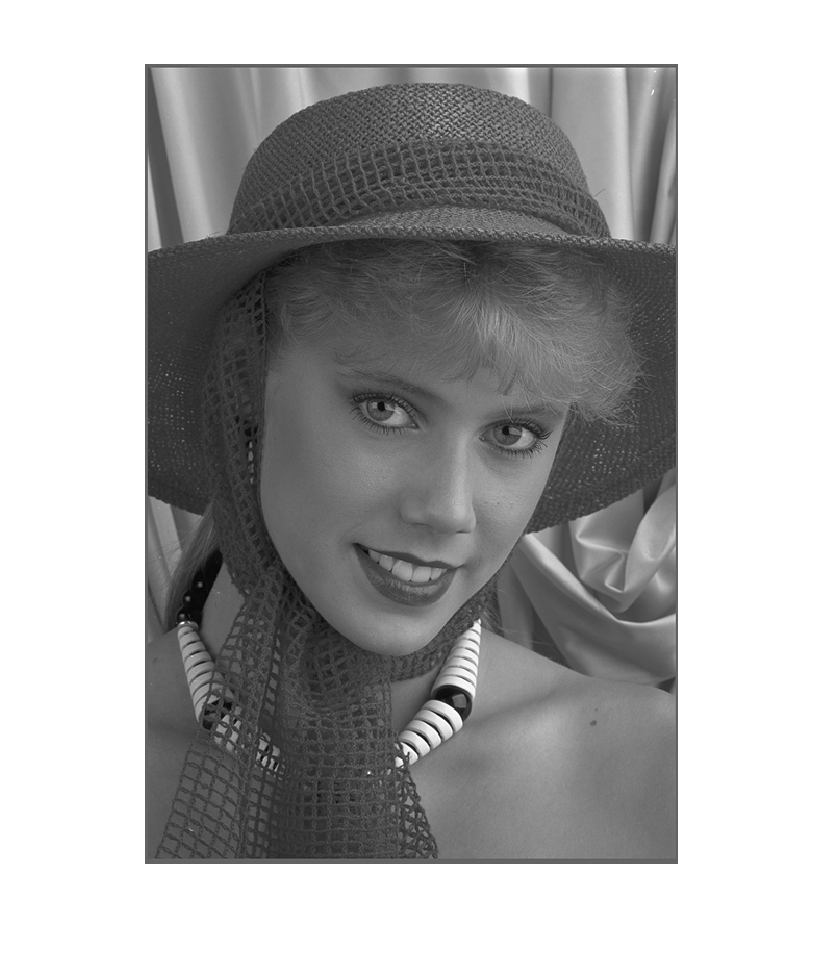
\includegraphics[height =3in]{imgo.eps}
	\caption{The original image}
	
	
	
\end{figure}
\begin{figure}[H]
	
	\centering
	\subfigure[\emph{img0.25.tif}]{
		
		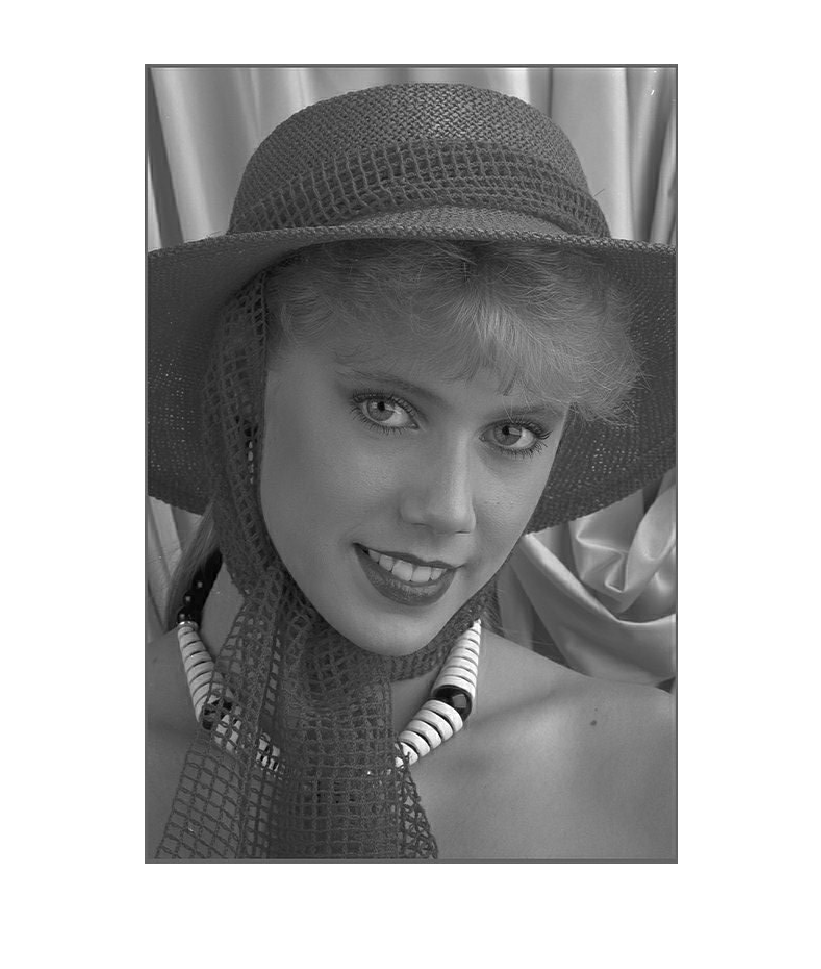
\includegraphics[width=2.5in]{img025.eps}}
	\hspace{0in} 
	\subfigure[\emph{img0.25d.tif}]{
		
		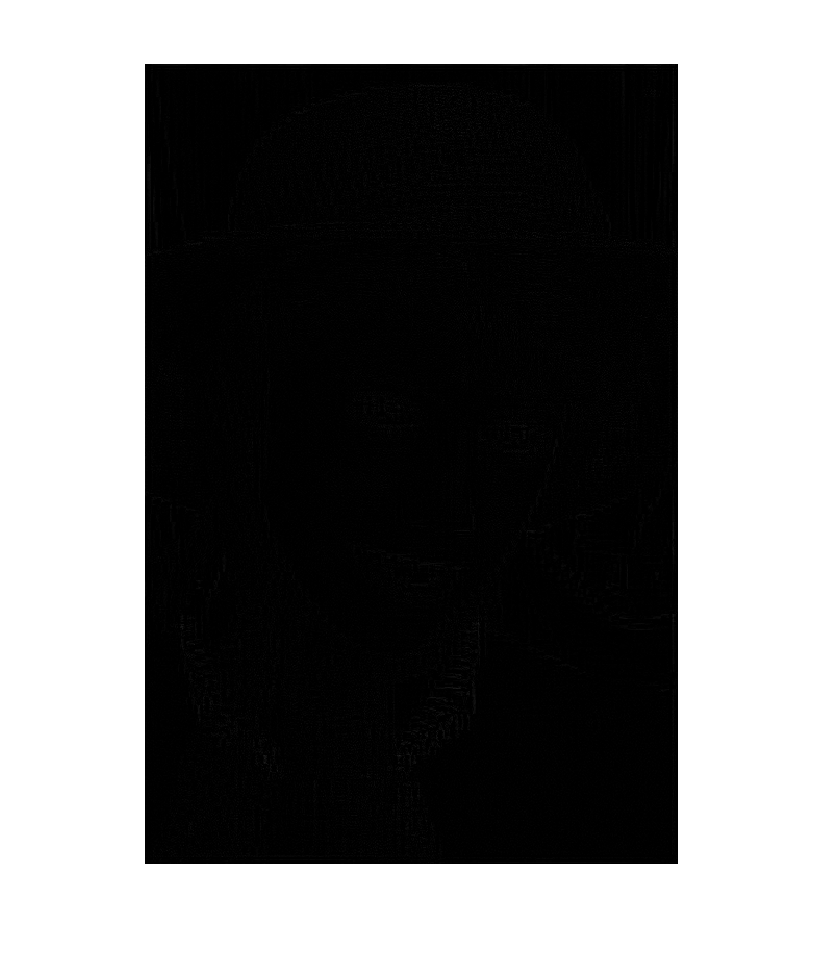
\includegraphics[width = 2.5in]{img025d.eps}}
	\hspace{0in} 
		\subfigure[\emph{img0/25Enhanced.tif}]{
		
		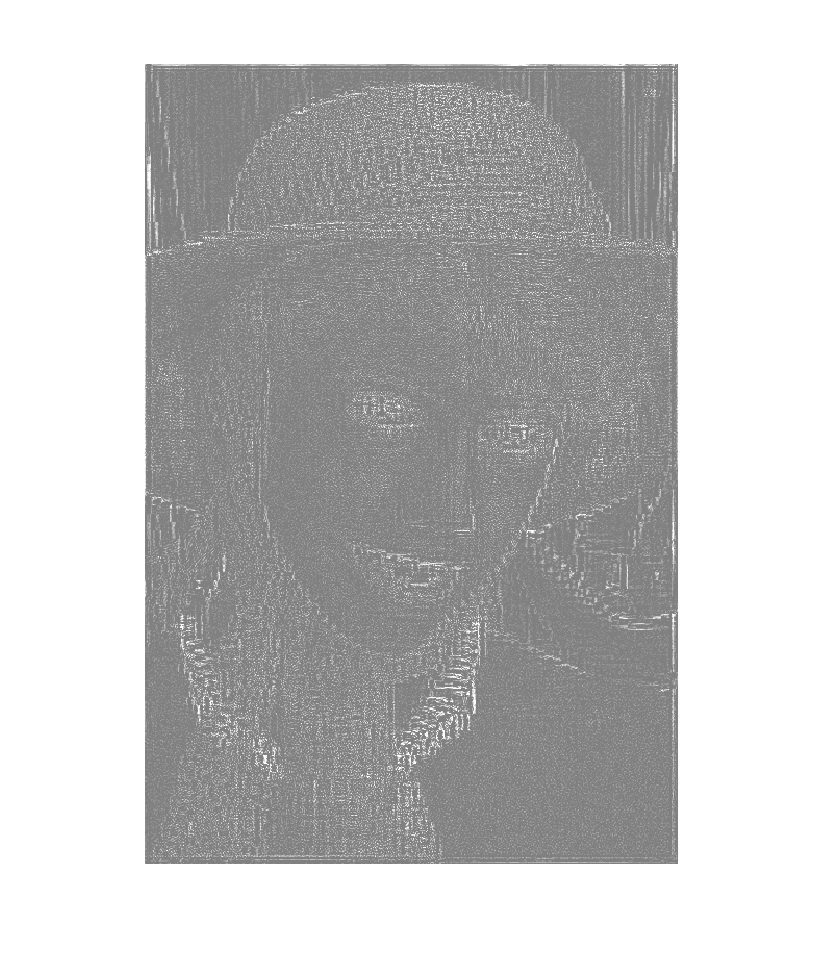
\includegraphics[width=2.5in]{img025e.eps}}
	\caption{Restored Image and the difference with a r of 0.25}
	
\end{figure}
\begin{figure}[H]
	
	\centering
	\subfigure[\emph{img1.tif}]{
		
		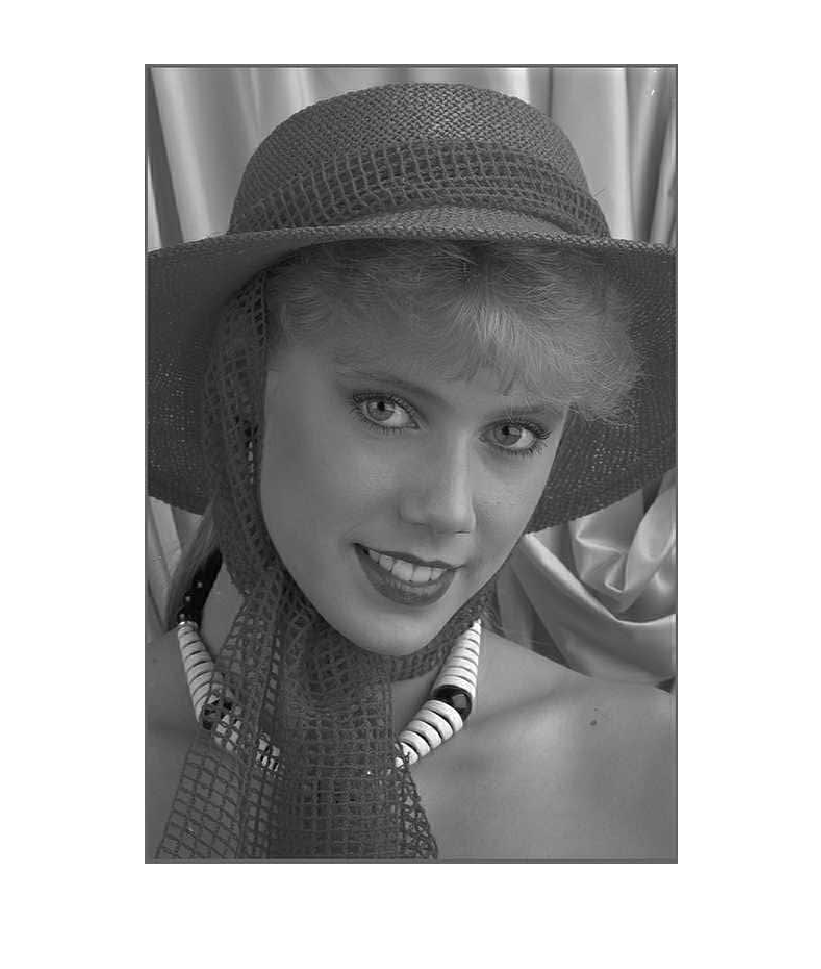
\includegraphics[width=2.5in]{img1.eps}}
	\hspace{0in} 
	\subfigure[\emph{img1d.tif}]{
		
		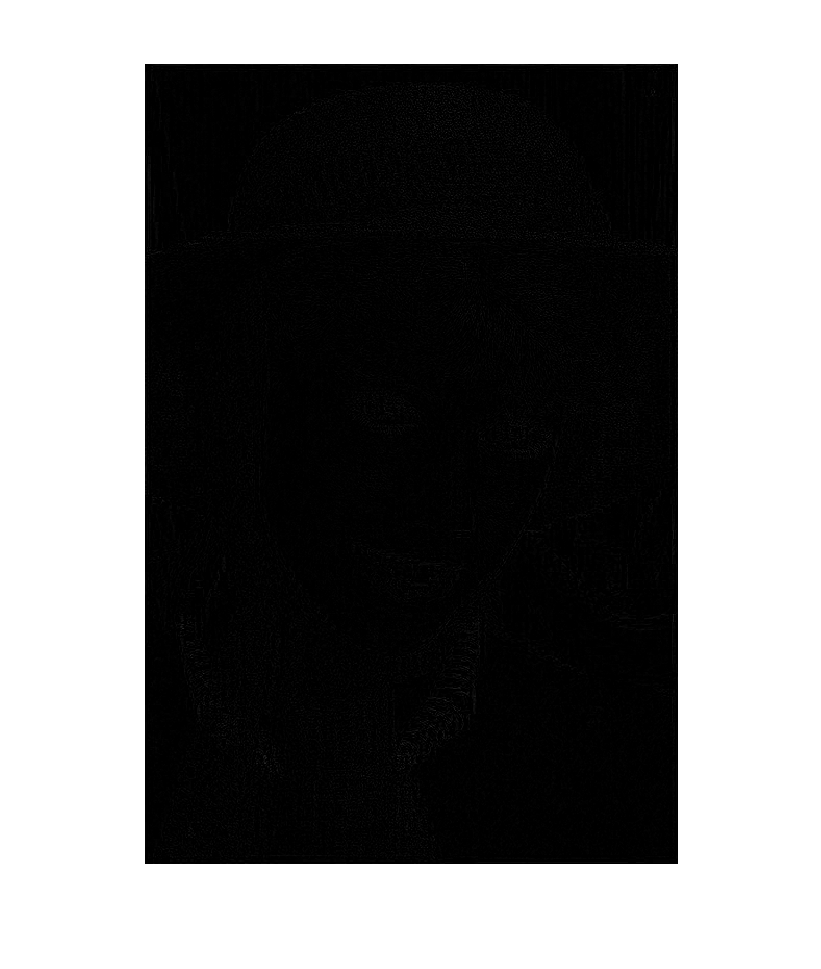
\includegraphics[width=2.5in]{img1d.eps}}
		\subfigure[\emph{img1Enhanced.tif}]{
		
		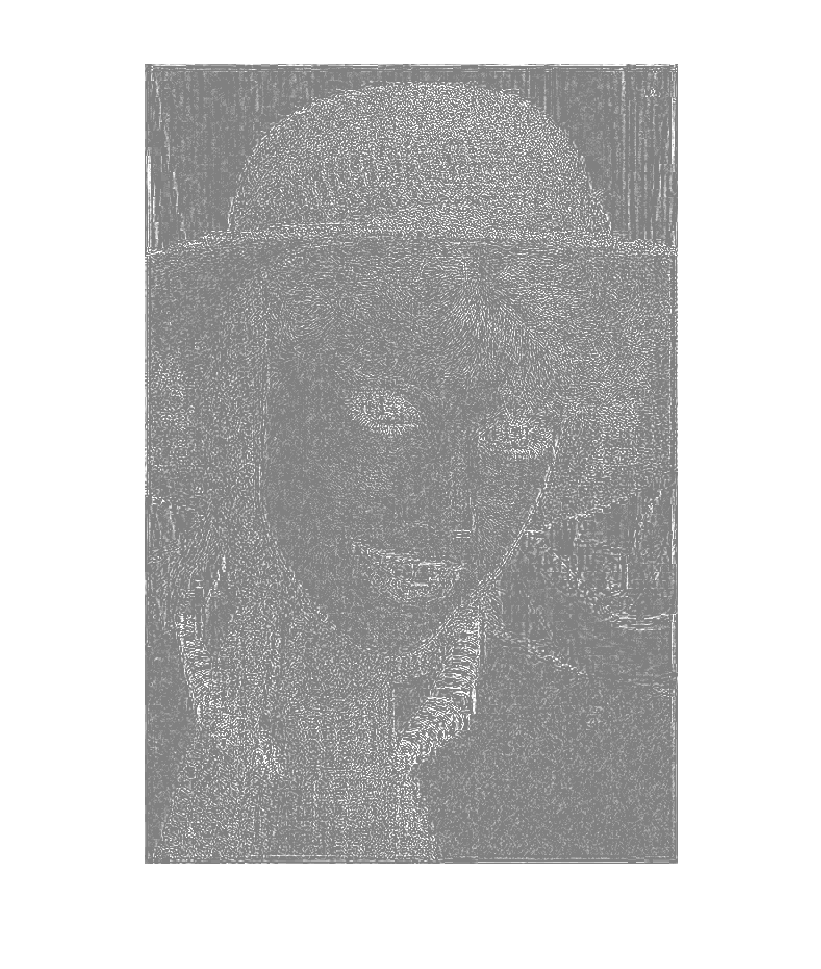
\includegraphics[width=2.5in]{img1e.eps}}
	\caption{Restored Image and the difference with a $\gamma$ of 1}
	
\end{figure}
\begin{figure}[H]
	
	\centering
	\subfigure[\emph{img4.tif}]{
		
		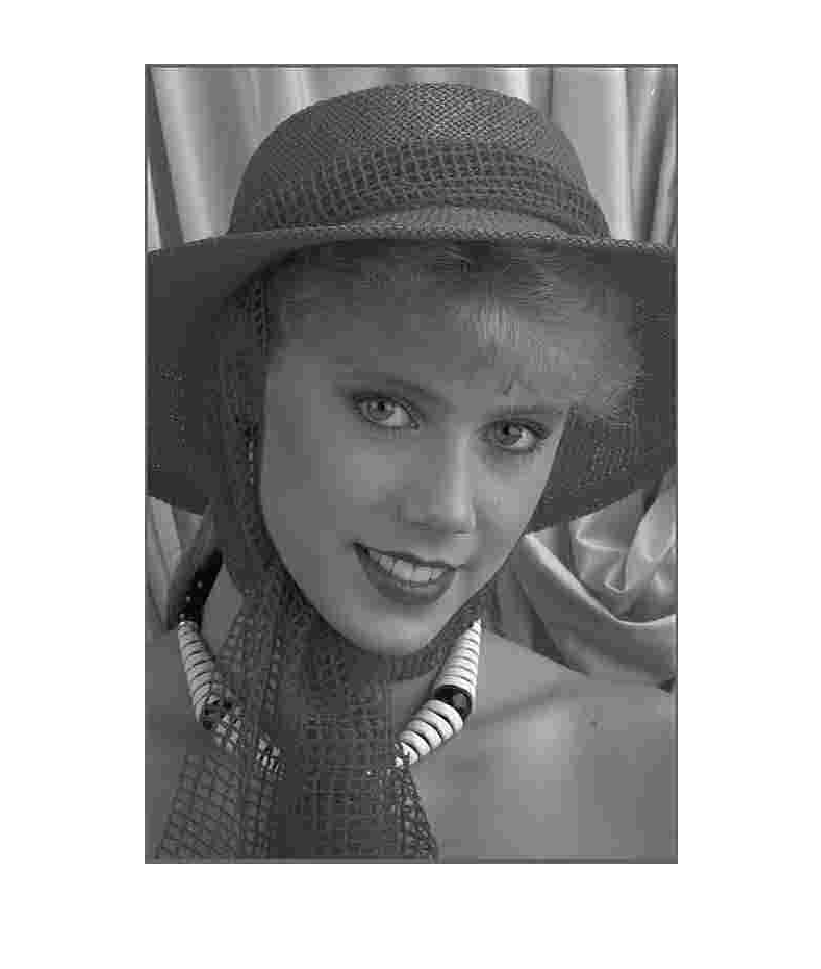
\includegraphics[width=2.5in]{img4.eps}}
	\hspace{0in} 
	\subfigure[\emph{img4d.tif}]{
		
		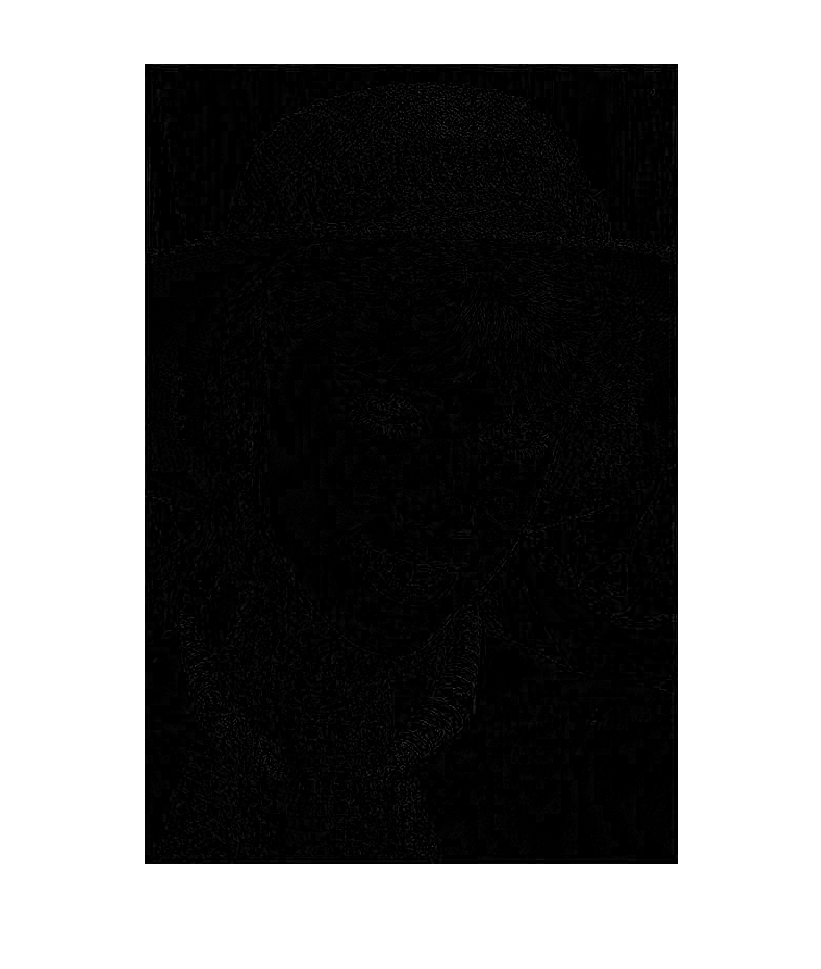
\includegraphics[width=2.5in]{img4d.eps}}
	\subfigure[\emph{img4Enhanced.tif}]{
		
		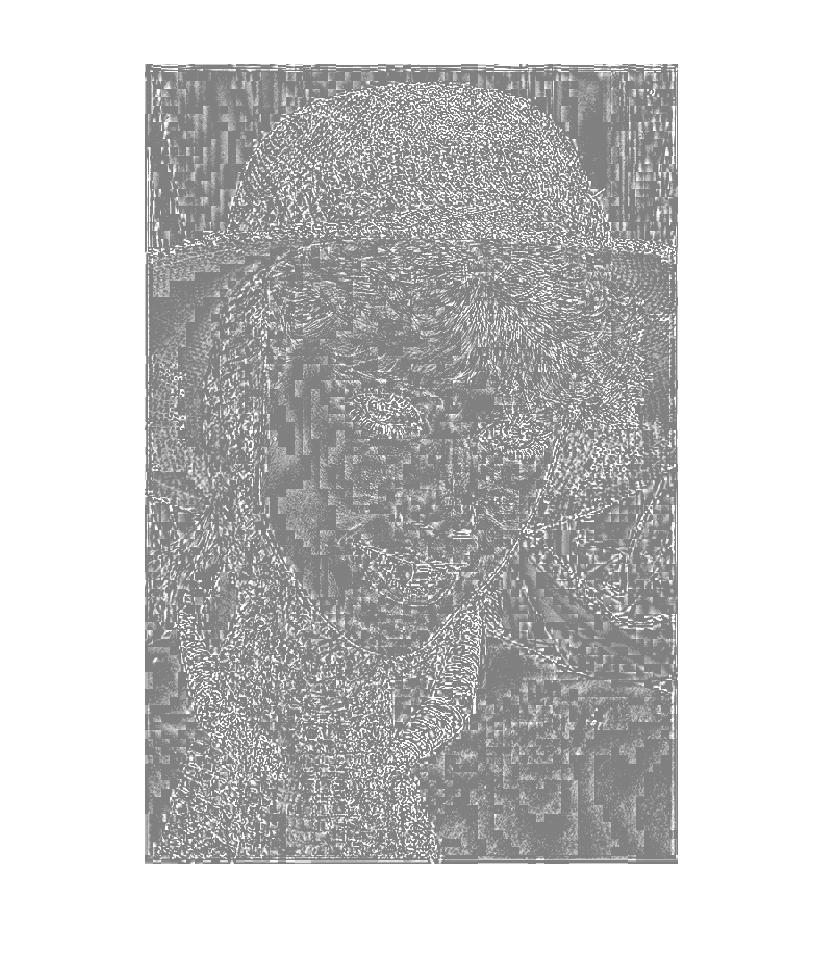
\includegraphics[width=2.5in]{img4e.eps}}
	
	\caption{Restored Image and the difference with a $\gamma$ of 4}
	
\end{figure}
\emph{PS: In this part, the error img was enhanced with a formula of 10 times multiply and adding 128 pixel gray value. }
\subsection{Comment on the Result}
According to the result, the $\gamma$ represent a quantization factor in the process. With the increasing of $\gamma$, the quantization blocks are bigger and the resolution decreases.

\section{Differential Encoding and the Zig-Zag Scan Pattern
}
To improve image quality and reduce bit rate, the DC coefficient is differentially encoded.
This means that, using a raster ordering of the blocks, only the difference between the current
and previous DC coefficients is coded.

\subsection{Result report} 
\begin{figure}[H]
	
	\centering
	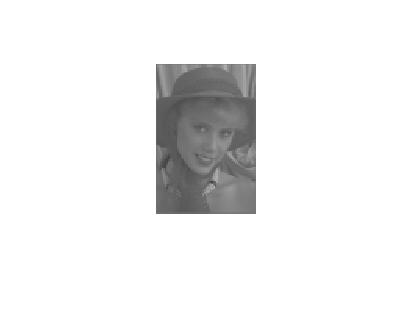
\includegraphics[height =3in]{DC.eps}
	\caption{The DC component formed image}
	
	
	
\end{figure}
This looks a little dizzy, like a resized form of the original image. this is probably because the image information is mainly stored in the DC components. 
\\
 
The DC components have the highest energy and represent the main information in the whole coding block. And in an image, nearby pixels are correlated. So, the adjacent DC components are correlated.
\begin{figure}[H]
	
	\centering
	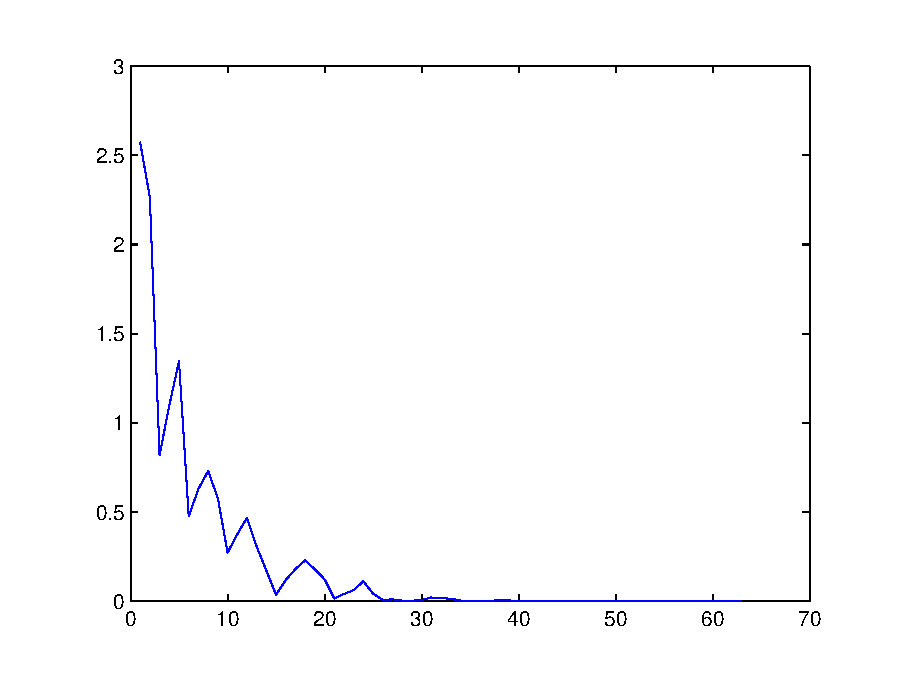
\includegraphics[height = 3in]{plot.eps}
	\caption{ plot of the mean value of the magnitude of the AC coefficients for $\gamma$ = 1.0.}
	
	
	
\end{figure}

In this figure, the mean value of magnitude of the AC coefficients goes down. This is probably because in one DCT block, the energy goes down when it goes far away from the upper-left corner. 
\subsection{Code Listing}
\begin{lstlisting}[frame=single]

I = imread('img03y.tif');
I = double(I);
I = I - 128;

gamma = 1;
fn = @(x) round(dct2(x.data,[8,8])./(Quant*gamma));
dct_blk = blockproc(I,[8,8],fn);

[r,c] = size(dct_blk);
DC = zeros(r/8,c/8);
AC = zeros(r*c/64,63);

for i = 0:r/8-1
for j = 0:c/8-1
DC(i+1,j+1) = dct_blk(i*8+1,j*8+1) + 128;
temp = dct_blk(i*8+1:i*8+8,j*8+1:j*8+8);
temp = temp(Zig);
AC(i*c/8 + j + 1,:) = temp(2:end);
end
end

DC = uint8(DC);
figure(1)
imshow(DC)
AC_mean = mean(abs(AC));
t = 1:63;
figure(2)
plot(t,AC_mean)


\end{lstlisting}
\section{Entropy Encoding of Coefficients}

In order to reduce the number of bits required to represent the quantized image, both the
differential DC and AC coefficients must be entropy encoded. To do this, JPEG uses two
basic encoding schemes, the \emph{Variable-Length Code} (VLC) and the \emph{Variable-Length Integer}
(VLI). The VLC encodes the number of bits used for each coefficient, and the VLI encodes
the signed integer efficiently.

\subsection{Subroutine Coding List} 
\subsubsection{BitSize}
\lstset{ %
	backgroundcolor=\color{white},   % choose the background color; you must add \usepackage{color} or \usepackage{xcolor}; should come as last argument
	basicstyle=\footnotesize,        % the size of the fonts that are used for the code
	breakatwhitespace=false,         % sets if automatic breaks should only happen at whitespace
	breaklines=true,                 % sets automatic line breaking
	captionpos=b,                    % sets the caption-position to bottom
	commentstyle=\color{mygreen},    % comment style
	deletekeywords={...},            % if you want to delete keywords from the given language
	escapeinside={\%*}{*)},          % if you want to add LaTeX within your code
	extendedchars=true,              % lets you use non-ASCII characters; for 8-bits encodings only, does not work with UTF-8
	frame=single,	                   % adds a frame around the code
	keepspaces=true,                 % keeps spaces in text, useful for keeping indentation of code (possibly needs columns=flexible)
	keywordstyle=\color{blue},       % keyword style
	language=Octave,                 % the language of the code
	morekeywords={*,...},           % if you want to add more keywords to the set
	numbers=left,                    % where to put the line-numbers; possible values are (none, left, right)
	numbersep=5pt,                   % how far the line-numbers are from the code
	numberstyle=\tiny\color{mygray}, % the style that is used for the line-numbers
	rulecolor=\color{black},         % if not set, the frame-color may be changed on line-breaks within not-black text (e.g. comments (green here))
	showspaces=false,                % show spaces everywhere adding particular underscores; it overrides 'showstringspaces'
	showstringspaces=false,          % underline spaces within strings only
	showtabs=false,                  % show tabs within strings adding particular underscores
	stepnumber=2,                    % the step between two line-numbers. If it's 1, each line will be numbered
	stringstyle=\color{mymauve},     % string literal style
	tabsize=2,	                   % sets default tabsize to 2 spaces
	title=\lstname                   % show the filename of files included with \lstinputlisting; also try caption instead of title
}
\begin{lstlisting}[frame=single]

int BitSize(int value)
{
int bitsize=0;

if(value<0)
value=-value;   

while( (value-(1<<bitsize) >= 0) && (bitsize<16) )
bitsize++;

return(bitsize);
}

\end{lstlisting}
\subsubsection{VLI\_encode}
\begin{lstlisting}[frame=single]

void VLI_encode(int bitsize, int value, char *block_code)
{
int k;
char buffer[17];  /* max VLI code length should be 16 */


if(bitsize>16)
fprintf(stderr,"Error");

if(value<0)
value = value-1;  

for(k=bitsize; k>0; k--){
if( (value & (1<<(k-1))) == 0)  
buffer[bitsize-k]='0';
else
buffer[bitsize-k]='1'; 
}
buffer[bitsize]='\0';  
strcat(block_code,buffer);
}  
\end{lstlisting}
\subsubsection{ZigZag}
\begin{lstlisting}[frame=single]

void ZigZag(int ** img, int y, int x, int *zigline) {
fprintf(stdout, "in ZigZag()\n");
int i, j;

for (i = 0; i < 8; i++) {
for (j = 0; j < 8; j++) {
zigline[Zig[i][j]] = img[y+i][x+j];
}
}
}
\end{lstlisting}

\subsubsection{DC\_encoder}
\begin{lstlisting}
void DC_encode(int dc_value, int prev_value, char *block_code) {
int diff, size;

diff = dc_value - prev_value;
size = BitSize(diff);

strcat(block_code, dcHuffman.code[size]);
VLI_encode(size, diff, block_code);
}
\end{lstlisting}
\subsubsection{AC\_encoder}
\begin{lstlisting}
	int idx = 1;
int zerocnt = 0;
int bitsize;

while (idx < 64) {
if (zigzag[idx] == 0) {
zerocnt++;
} else {
for (; zerocnt > 15; zerocnt -= 16) {
strcat(block_code, acHuffman.code[15][0]);
}

bitsize = BitSize(zigzag[idx]);
strcat(block_code, acHuffman.code[zerocnt][bitsize]);
VLI_encode(bitsize, zigzag[idx], block_code);

zerocnt = 0;
}

idx++;
}
\end{lstlisting}
\subsubsection{Block\_encoder}
\begin{lstlisting}
void Block_encode(int prev_dc, int *zigzag, char *block_code)
{
DC_encode(zigzag[0],prev_dc,block_code);
AC_encode(zigzag,block_code);
}
\end{lstlisting}

\subsubsection{Convert\_encoder}
\begin{lstlisting}
int Convert_encode(char *block_code, unsigned char *byte_code) {
int len = strlen(block_code);
int bytes = len / 8;
int idx;
int i, j;

idx = 0;
for (i = 0; i < bytes; i++) {
for (j = 0; j < 8; j++) {
byte_code[idx] <<= 1;

if (block_code[i*8 + j] == '1') {
byte_code[idx]++;
}
}

if (byte_code[idx] == 0xff) {
byte_code[++idx] == 0x00;
bytes++;
}

idx++;
}

strcpy(block_code, block_code + len / 8 * 8);

return bytes;
}
\end{lstlisting}

\subsubsection{Zero\_pad}
\begin{lstlisting}
unsigned char Zero_pad(char *block_code)
{
unsigned char byte_value=0;
int k=0;
char mask;

while( block_code[k] != '\0' ) {
mask= 0x80 >> (k%8);         

if( block_code[k] == '1' )
byte_value |= mask;         

if( block_code[k] == '0' )
byte_value &= (~mask);      

k++;
}

return(byte_value);
}  
\end{lstlisting}

\subsection{Main Image Coding Program}
\begin{lstlisting}


#include <stdio.h>
#include <stdlib.h>
#include <string.h>

#include "Htables.h"
#include "JPEGdefs.h"
#include "allocate.h"


int main(int argc, char* argv[])
{
int  **input_img;  
FILE  *outfp;     
int    row;        /* height  */
int    column;     /* width  */
double gamma;      /* scaling parameter */
int temp, k,i,j;
char tempc[100];
int tempi[64];
int **img;
unsigned char byte_code[100];
unsigned char tempuc;

input_img = get_arguments(argc,argv,&row,&column,&gamma,&outfp) ;

if( gamma > 0 )
change_qtable(gamma) ;
else {
fprintf(stderr, "\nQuantizer scaling must be > 0.\n") ;
exit(-1) ;
}

jpeg_encode(input_img,row,column,outfp) ;

return 1 ;
}


void change_qtable(double scale)
{
int     i,j ;
double  val ;

for(i=0;i<8;i++){
for(j=0;j<8;j++){
val = Quant[i][j]*scale ;
/* w.r.t spec, Quant entry can be bigger than 16 bit */
Quant[i][j] = (val>65535) ? 65535 : (int)(val+0.5) ;
}
}
}


int **get_arguments(int argc,
char *argv[],
int *row,
int *col,
double *gamma,
FILE **fp ) 
{
/*  float    val ; */
FILE *   inp ;
short**  img ;
int  **  in_img ;
short    tmp ;
int      i,j ;

switch(argc){
case 0:
case 1:
case 2: 
case 3: usage(); exit(-1) ; break ; 
default:

sscanf(argv[1],"%lf",gamma) ;

*fp = fopen(argv[3],"wb") ;
if(*fp==NULL) {
fprintf(stderr,
"\n%s file error\n",argv[3]) ;
exit(-1) ;
}

inp = fopen(argv[2],"rb") ;
if( inp == NULL ) {
fprintf(stderr,
"\n%s open error\n",argv[2]) ;
exit(-1) ;
}

fread(&tmp,sizeof(short),1,inp) ;
*row = (int) tmp ;
fread(&tmp,sizeof(short),1,inp) ;
*col = (int) tmp ;

img = (short **)get_img(*col,*row,sizeof(short)) ;
fread(img[0],sizeof(short),*col**row,inp) ;
fclose(inp) ;

break ;
}

in_img = (int **)get_img(*col,*row,sizeof(int)) ;
for( i=0 ; i<*row; i++ ){
for( j=0 ; j<*col; j++ ){
in_img[i][j] = (int) img[i][j] ;
}
}
free_img((void**)img) ;
return( in_img ) ;
}


void jpeg_encode(int **img, int h, int w, FILE *jpgp)
{
int    x, y, i, j, length ; 
int    prev_dc = 0 ;
unsigned char val ;
static int    zigline[64] ;
static char   block_code[8192] = {0} ;
static unsigned char byte_code[1024] ;

printf("\n JPEG encode starts...") ;
/* JPEG header writes */
put_header(w,h,Quant,jpgp) ;

printf("\n Header written...\n Image size %d row  %d column\n",h,w) ;
/* Normal block processing */
for( y = 0 ; y < h ; y += 8) {
for( x = 0 ; x < w ; x += 8 ){
/* read up 8x8 block */
ZigZag(img,y,x,zigline) ;

Block_encode(prev_dc,zigline,block_code) ;


prev_dc = zigline[0] ;
length = Convert_encode(block_code,byte_code) ;
fwrite(byte_code,sizeof(char),length,jpgp) ;
}
printf("\r (%d)th row processing   ",y) ;
}
printf("\nEncode done.\n") ;

if( strlen(block_code) ){
val = Zero_pad(block_code) ;
fwrite(&val,sizeof(char),1,jpgp) ;
}

put_tail(jpgp) ;
fclose(jpgp) ;
free_img((void **)img) ;
}

\end{lstlisting}
\subsubsection{Result Report}
\begin{figure}[H]
	
	\centering
	\subfigure[\emph{output\_.25.jpg}]{
		
		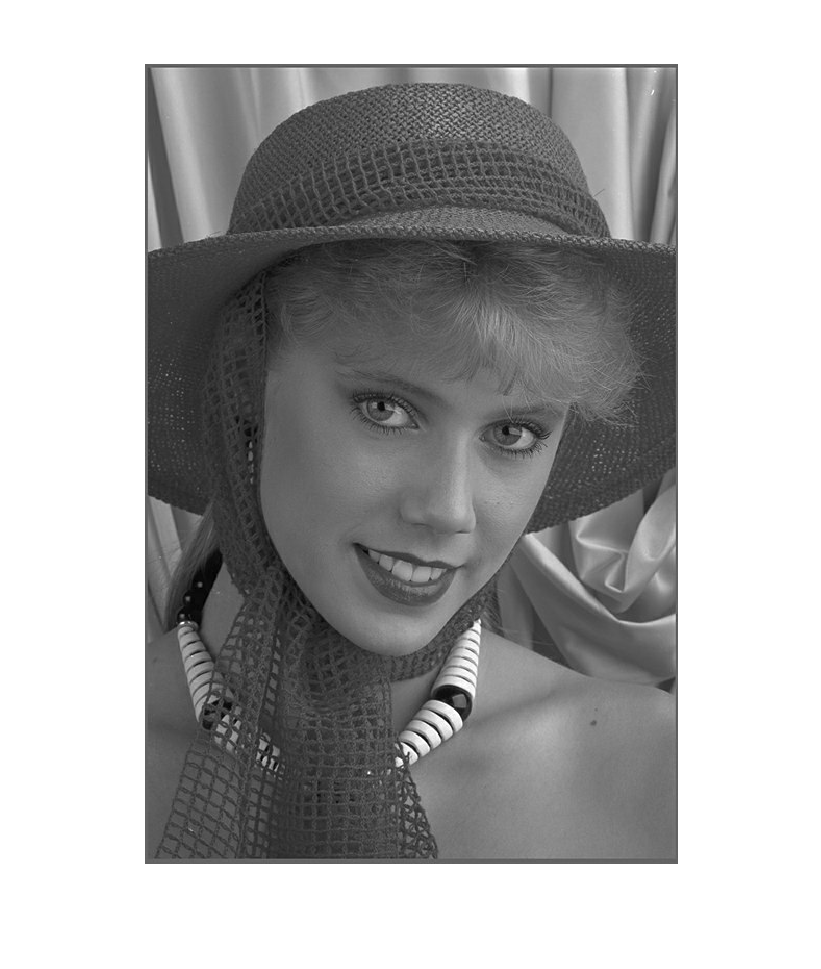
\includegraphics[width=2.5in]{o025.eps}}
	\hspace{0in} 
	\subfigure[\emph{img\_1.jpg}]{
		
		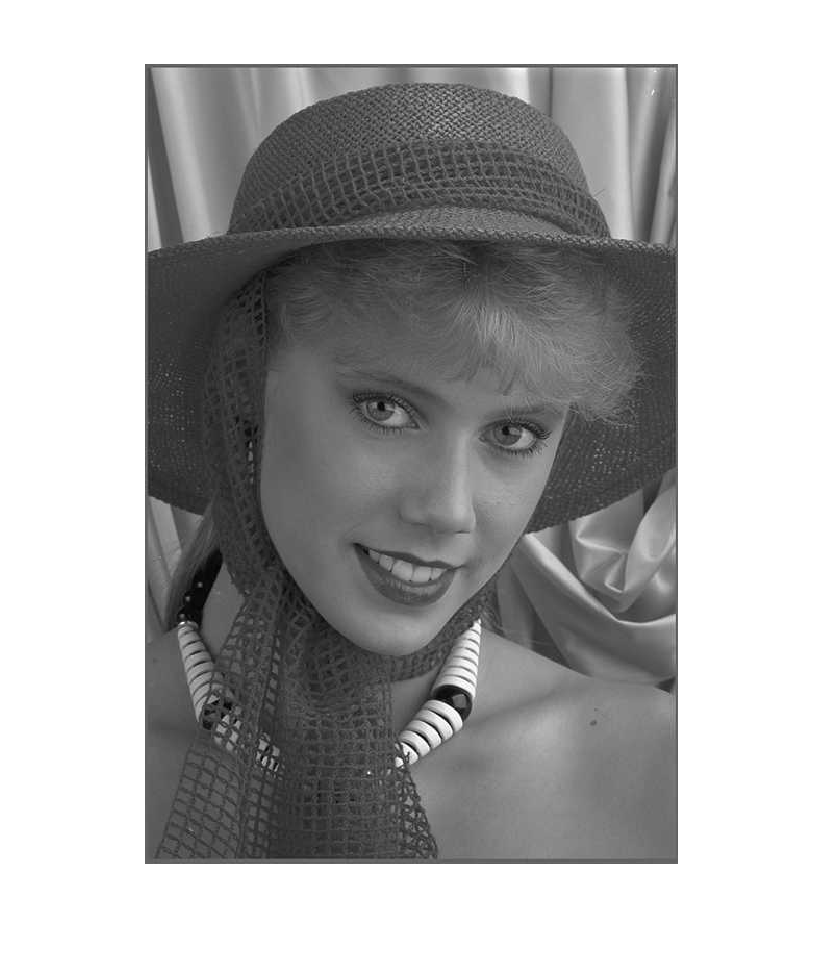
\includegraphics[width = 2.5in]{o1.eps}}
	\hspace{0in} 
	\subfigure[\emph{img\_4.jpg}]{
		
		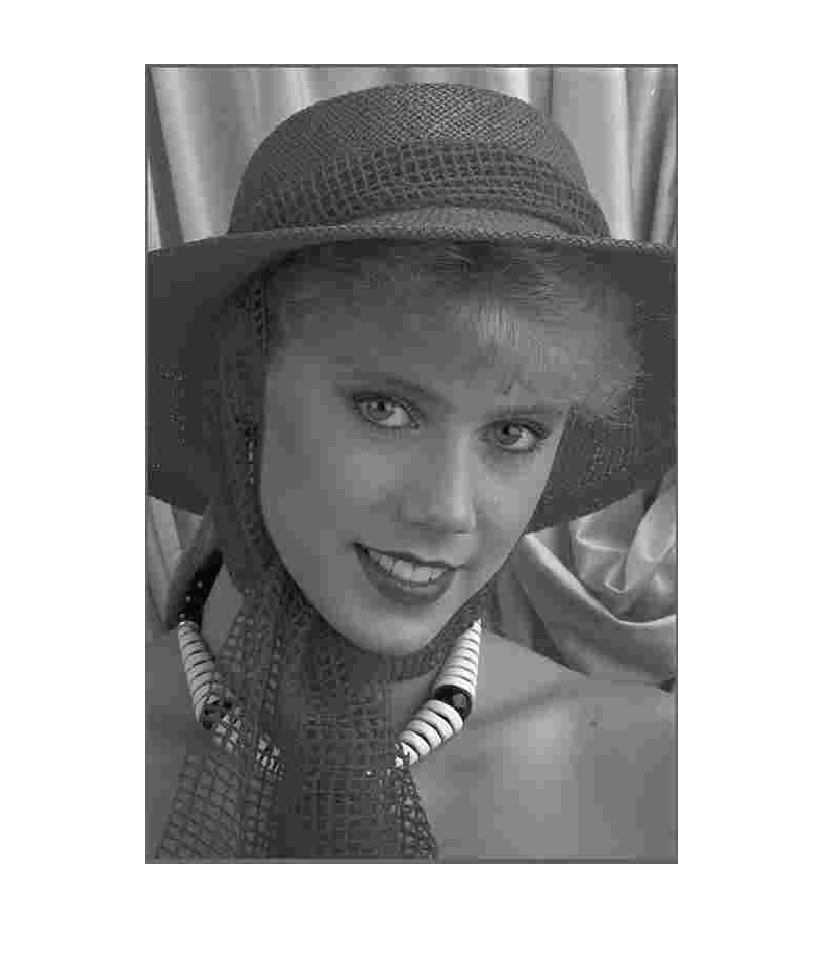
\includegraphics[width=2.5in]{o4.eps}}
	\caption{Restored Image and the difference with a r of 0.25, 1 and 4}
	
\end{figure}
\end{document}